\chapter{Horizons, équation d’état et énergie du vide}

\section{Référentiel privilégié, récession supraluminique et horizon}

Le fond diffus cosmologique définit bien un référentiel particulier. Dans le référentiel où ce rayonnement paraît isotrope, les galaxies proches sont également, en moyenne, au repos. Si nous nous déplaçons par rapport au fond diffus, les photons venant de l’avant sont décalés vers les hautes énergies par effet Doppler, tandis que ceux venant de l’arrière sont décalés vers les basses énergies. Le référentiel privilégié est celui dans lequel le fond diffus micro-onde paraît isotrope ; c’est aussi, en moyenne, le référentiel dans lequel les galaxies locales sont au repos.

\begin{classroomqa}\lecturetimestamp{00:00:25}\audiencequestion{La longueur d’onde apparente du rayonnement cosmique dépend-elle du mouvement de l’observateur, et cela implique-t-il l’existence d’un référentiel privilégié ?}\lecturerresponse{Oui. Le mouvement par rapport au fond diffus micro-onde produit une anisotropie Doppler ; il existe donc un référentiel cosmologique privilégié : celui dans lequel le fond diffus micro-onde paraît isotrope. C’est aussi, en moyenne, le référentiel dans lequel les galaxies locales sont au repos.}\end{classroomqa}

Une deuxième question porte sur les vitesses de récession. La loi de Hubble indique que les galaxies suffisamment lointaines s’éloignent selon
\begin{equation}
v = H d .
\end{equation}
Pour une valeur assez grande de \(d\), cette vitesse de récession dépasse celle de la lumière. Cela ne contredit pas la relativité, car l’interdiction est locale : un objet ne peut pas dépasser un autre, juste devant nous, à une vitesse supérieure à celle de la lumière. L’énoncé concernant les galaxies lointaines porte sur la géométrie entre des lieux très éloignés.

\begin{classroomqa}\lecturetimestamp{00:04:48}\audiencequestion{Deux galaxies peuvent-elles avoir une vitesse relative supérieure à \(c\) ?}\lecturerresponse{Oui, si elles sont suffisamment éloignées. La récession de Hubble peut dépasser la vitesse de la lumière sans violer la relativité locale ; l’endroit où la vitesse de récession atteint \(c\) est un horizon.}\end{classroomqa}

Dès que la récession atteint la vitesse de la lumière, les signaux envoyés vers nous ne progressent plus globalement vers nous. Le rayon se déplace toujours localement à la vitesse limite, mais la distance qu’il doit parcourir augmente trop rapidement.

\begin{classroomqa}\lecturetimestamp{00:07:03}\audiencequestion{Un rayon lumineux envoyé dans le sens opposé ne se déplacerait-il pas quand même vers nous ?}\lecturerresponse{Localement, si, mais l’espace s’étend plus vite que le rayon ne peut la parcourir. Le rayon se déplace à la vitesse limite par rapport aux points voisins, tandis que la distance totale qui nous en sépare continue d’augmenter.}\end{classroomqa}

\section{La métrique en expansion et l’analogie de la ligne}

Une image utile est celle d’une ligne unidimensionnelle. Imaginons une ligne constituée d’atomes. Si l’on étire une ligne matérielle ordinaire, elle finit par se rompre. Modifions maintenant l’image : chaque fois que des atomes voisins s’écartent trop, nous en insérons un autre entre eux. La ligne continue de s’allonger, mais ses propriétés locales ne se diluent pas.

\begin{figure}\centering
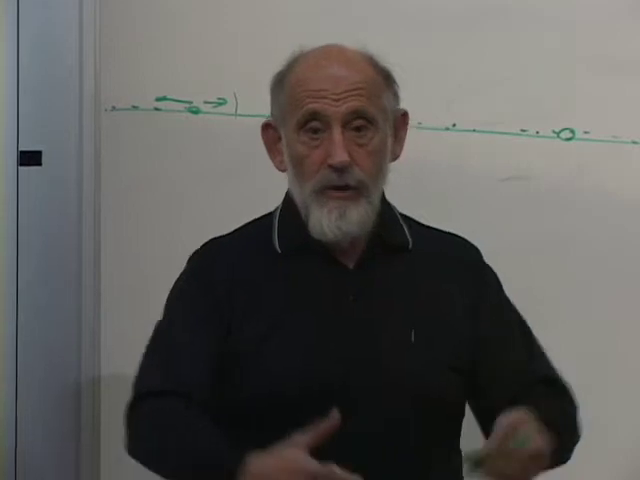
\includegraphics[width=0.60\textwidth]{lecture_04_figure_02.png}\caption{Ligne unidimensionnelle servant à représenter une métrique en expansion.}\end{figure}

Dans cette image, il existe toujours une vitesse limite de propagation des signaux à l’échelle locale, tout comme le son a une vitesse limite sur une ligne ordinaire. La règle est locale : une perturbation ne peut dépasser cette vitesse par rapport aux points voisins. Pourtant, si la ligne est suffisamment longue et que de nouveaux points sont insérés assez rapidement, des régions suffisamment éloignées s’éloignent si vite qu’aucun signal ne peut jamais revenir.

La composition des vitesses en relativité restreinte ne raconte donc qu’une partie de l’histoire. Elle s’applique localement, lorsque des observateurs se croisent au même endroit. Ce n’est pas l’outil approprié pour décrire des galaxies très éloignées dans une géométrie en expansion.

\begin{classroomqa}\lecturetimestamp{00:09:42}\audiencequestion{La loi ordinaire de composition relativiste des vitesses s’applique-t-elle encore dans cette situation ?}\lecturerresponse{Localement, en un point, oui. Si des observateurs se croisent les uns après les autres, la règle habituelle de la relativité restreinte s’applique. Mais elle ne convient pas pour décrire une récession supraluminique entre des régions très éloignées \(c\) ; il faut alors revenir à la géométrie de l’espace en expansion.}\end{classroomqa}

La même image donne une explication simple du décalage vers le rouge. Traçons une onde sur la ligne. Quand celle-ci s’étend, la longueur d’onde s’allonge avec elle. Dans une géométrie en expansion, il ne s’agit pas seulement d’une image évocatrice. Les équations d’onde en espace-temps en expansion produisent réellement des longueurs d’onde étirées.

\begin{classroomqa}\lecturetimestamp{00:14:42}\audiencequestion{L’affirmation selon laquelle une onde s’étire avec l’Univers est-elle théorique, empirique, ou les deux ?}\lecturerresponse{C’est une conséquence théorique de la propagation des ondes dans un espace-temps en expansion, et les observations astronomiques la confirment également.}\end{classroomqa}

Cette image ne représente pas un élastique. Un élastique s’amincit quand on l’étire, et une personne vivant dans un tel milieu verrait ses propriétés locales changer. Ici, les propriétés locales restent les mêmes tandis que l’échelle des distances globales augmente.

\section{Dernière diffusion et Univers observable}

L’horizon est le lieu où la récession atteint la vitesse de la lumière. La surface de dernière diffusion se trouve légèrement à l’intérieur de celui-ci. Un signal émis depuis l’horizon subirait un décalage vers le rouge sans borne ; celui du rayonnement de dernière diffusion est immense, mais fini.

\begin{classroomqa}\lecturetimestamp{00:17:53}\audiencequestion{Quel est le lien entre la récession supraluminique, la surface de dernière diffusion et l’Univers observable ?}\lecturerresponse{L’horizon est le lieu où la récession atteint la vitesse de la lumière. La surface de dernière diffusion se trouve légèrement à l’intérieur, car son décalage vers le rouge est énorme, mais fini. En pratique, elle marque le bord de l’Univers observable.}\end{classroomqa}

Le décalage vers le rouge du rayonnement de dernière diffusion est de l’ordre d’un facteur \(10^3\). Il est déjà si grand que, à bien des égards, la surface de dernière diffusion est très proche de l’horizon. L’Univers observable est la partie de l’Univers d’où la lumière peut nous parvenir.

Aux temps tardifs, l’expansion tend vers le régime dominé par le vide. Alors, la quantité de Hubble tend vers une constante, l’horizon tend vers une taille fixe, et les galaxies comme le rayonnement micro-onde disparaissent progressivement de notre champ d’observation.

\begin{classroomqa}\lecturetimestamp{00:22:43}\audiencequestion{Puisque \(H\) varie au cours du temps, la distance de l’horizon varie-t-elle, et le fond diffus micro-onde finira-t-il par disparaître ?}\lecturerresponse{Aux temps tardifs, \(H\) tend vers une constante, de sorte que l’horizon tend vers une distance fixe. Le fond diffus micro-onde continue de s’étirer, de se refroidir et de s’affaiblir. Les galaxies lointaines franchissent elles aussi l’horizon et disparaissent de notre champ d’observation.}\end{classroomqa}

Seules les structures déjà liées gravitationnellement restent visibles. Le système solaire ne se disloque pas, pas plus que la galaxie, mais l’Univers à grande échelle devient une île isolée.

\section{Équation fondamentale de l’expansion et ses trois composantes}

L’équation fondamentale de l’expansion s’écrit maintenant
\begin{equation}
\left(\frac{\dot a}{a}\right)^2 = \frac{8\pi G}{3}\rho ,
\qquad c=1 .
\end{equation}
Ici, \(a(t)\) est le facteur d’échelle et \(\rho\) la densité d’énergie totale.

\begin{figure}\centering
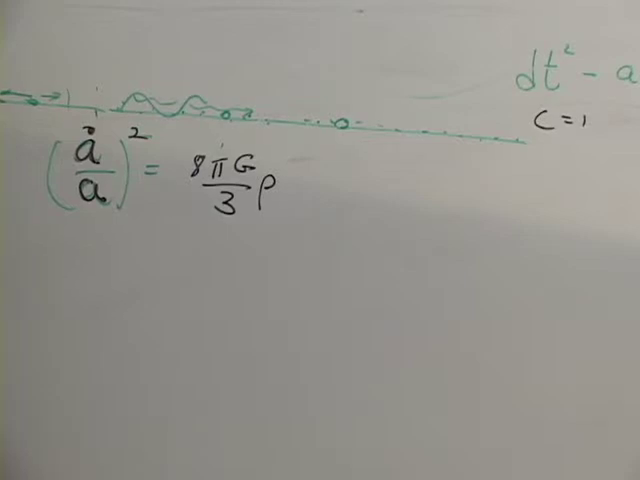
\includegraphics[width=0.74\textwidth]{lecture_04_figure_03.png}\caption{Équation fondamentale de l’expansion et analogie de la ligne unidimensionnelle.}\end{figure}

Trois composantes jouent un rôle important dans la dynamique.

Pour la matière,
\begin{equation}
\rho=\frac{\text{const.}}{a^3},
\qquad
a(t)\sim t^{2/3}.
\end{equation}
C’est le cas d’objets massifs qui suivent l’expansion globale et sont essentiellement au repos dans le référentiel comobile.

Pour le rayonnement,
\begin{equation}
\rho=\frac{\text{const.}}{a^4},
\qquad
a(t)\sim t^{1/2}.
\end{equation}
La puissance supplémentaire de \(a\) vient du décalage vers le rouge de chaque photon à mesure que l’Univers s’étend.

Il y a aussi
\begin{equation}
\rho_0=\text{constant},
\end{equation}
l’énergie du vide, également appelée énergie noire ou, à des facteurs numériques conventionnels près, constante cosmologique. Cette composante ne se dilue pas du tout.

L’étape suivante consiste à relier la densité d’énergie à la pression.

\section{Pression du rayonnement et matière froide}

Commençons par le rayonnement. Considérons une boîte unidimensionnelle, simplement un segment de longueur \(L\), contenant des photons qui rebondissent d’un bout à l’autre. En une dimension, force et pression sont pratiquement équivalentes.

Considérons un photon de quantité de mouvement de norme \(p\). Lorsqu’il se réfléchit sur une paroi, sa quantité de mouvement varie de
\begin{equation}
\Delta p = 2p.
\end{equation}
Le temps entre deux collisions successives avec la même paroi est
\begin{equation}
\Delta t = \frac{2L}{c}.
\end{equation}
La force moyenne exercée sur la paroi est donc
\begin{equation}
F=\frac{\Delta p}{\Delta t}=\frac{pc}{L}.
\end{equation}
Pour un photon,
\begin{equation}
E=pc,
\end{equation}
d’où
\begin{equation}
F=\frac{E}{L}.
\end{equation}
L’énergie divisée par la longueur correspond à la densité d’énergie en une dimension. Dans ce cas unidimensionnel,
\begin{equation}
P=\rho .
\end{equation}

Avec de nombreux photons, la même relation reste valable après moyennage. La force totale est simplement l’énergie totale par unité de longueur.

Passons maintenant à trois dimensions. Si tous les photons se déplaçaient le long d’un seul axe, ils exerceraient une pression sur une paire de faces et aucune sur les autres. Ce cas est volontairement erroné, mais il montre immédiatement ce qu’il faut corriger. Dans un bain isotrope, la quantité de mouvement est répartie dans toutes les directions. En moyenne, un tiers de la densité d’énergie contribue à chaque composante de la pression. On obtient
\begin{equation}
P=\frac{\rho}{3}.
\end{equation}

Pour la matière froide, la réponse est différente. Considérons une boîte comobile, petite région qui se déplace avec le flot de l’Univers. Les particules qu’elle contient portent de l’énergie, mais si elles sont au repos par rapport à la boîte, elles ne heurtent pas ses parois. La pression est donc
\begin{equation}
P=0.
\end{equation}

\begin{figure}\centering
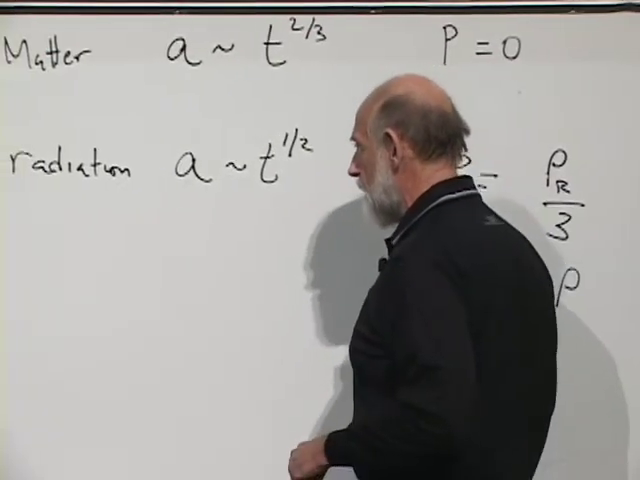
\includegraphics[width=0.74\textwidth]{lecture_04_figure_04.png}\caption{Matière et rayonnement : \(a\sim t^{2/3}\), \(P=0\), et \(a\sim t^{1/2}\), \(P=\rho/3\).}\end{figure}

Le récapitulatif au tableau est
\begin{align}
\text{matter:}\qquad & a(t)\sim t^{2/3}, \qquad P=0,\\
\text{radiation:}\qquad & a(t)\sim t^{1/2}, \qquad P=\frac{\rho}{3}.
\end{align}

\begin{classroomqa}\lecturetimestamp{00:54:27}\audiencequestion{Dans l’Univers en expansion, les particules ne s’éloignent-elles pas réellement les unes des autres ?}\lecturerresponse{Si, mais l’argument sur la pression s’applique à une boîte comobile infinitésimale. À cette échelle locale, le raisonnement thermodynamique reste valable.}\end{classroomqa}

\section{L’équation d’état}

On suppose que la pression est proportionnelle à la densité d’énergie,
\begin{equation}
P=w\rho .
\end{equation}
Au tableau, le même paramètre est noté \(\omega\). Pour les deux cas fondamentaux,
\begin{equation}
w=0 \quad \text{for cold matter},
\qquad
w=\frac{1}{3} \quad \text{for radiation}.
\end{equation}

Des cas intermédiaires sont possibles. Les valeurs comprises entre \(0\) et \(1/3\) décrivent une matière qui n’est ni complètement froide ni entièrement relativiste. La matière noire chaude en est l’exemple mentionné ici.

\begin{figure}\centering
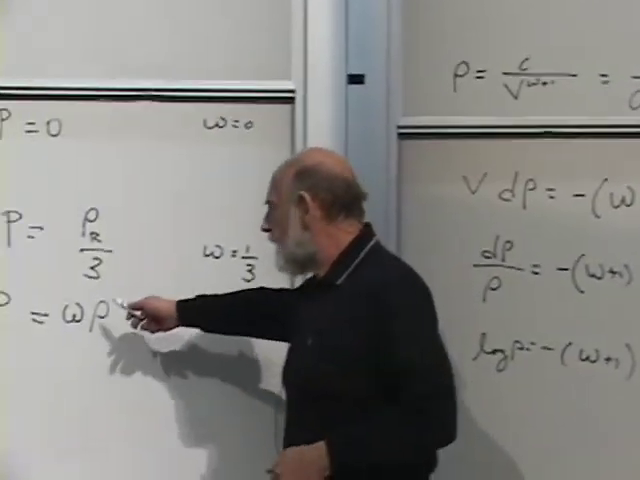
\includegraphics[width=0.74\textwidth]{lecture_04_figure_05.png}\caption{Équation d’état \(P=\omega\rho\) et argument d’échelle de la densité.}\end{figure}

La question suivante est de savoir si \(w\) détermine la dépendance de \(\rho\) en fonction de \(a\). La réponse vient d’une identité thermodynamique.

Considérons une boîte de volume \(V\). Si son contenu exerce une pression \(P\), alors, lorsque la boîte se dilate de \(dV\), le travail effectué sur ses parois est
\begin{equation}
dE=-P\,dV.
\end{equation}
Écrivons maintenant l’énergie sous la forme
\begin{equation}
E=\rho V.
\end{equation}
Sa différentielle est
\begin{equation}
dE=\rho\,dV+V\,d\rho .
\end{equation}
En égalant les deux expressions, on obtient
\begin{equation}
\rho\,dV+V\,d\rho=-P\,dV,
\end{equation}
soit
\begin{equation}
V\,d\rho=-(\rho+P)\,dV.
\end{equation}
En utilisant \(P=w\rho\),
\begin{equation}
V\,d\rho=-(1+w)\rho\,dV.
\end{equation}
Divisons par \(\rho V\) :
\begin{equation}
\frac{d\rho}{\rho}=-(1+w)\frac{dV}{V}.
\end{equation}
En intégrant,
\begin{equation}
\rho \propto V^{-(1+w)}.
\end{equation}
Pour une boîte cosmologique comobile,
\begin{equation}
V\propto a^3,
\end{equation}
et donc
\begin{equation}
\rho \propto a^{-3(1+w)}.
\end{equation}

On retrouve immédiatement les cas précédents :
\begin{align}
w=0 &\Longrightarrow \rho \propto a^{-3},\\
w=\frac{1}{3} &\Longrightarrow \rho \propto a^{-4}.
\end{align}

Voilà pourquoi \(w\) est important. Une fois \(\rho(a)\) connue, on peut la réintroduire dans l’équation de Friedmann. On essaie alors une loi de puissance \(a\sim t^\alpha\) et on détermine comment l’Univers se dilate pour cette équation d’état.

\section{Énergie du vide et pression négative}

Un cas particulier se comporte différemment :
\begin{equation}
w=-1.
\end{equation}
Alors
\begin{equation}
1+w=0,
\end{equation}
si bien que l’exposant s’annule et que
\begin{equation}
\rho=\rho_0=\text{constant}.
\end{equation}
La pression correspondante est
\begin{equation}
P=-\rho .
\end{equation}

La pression négative n’a rien de mystérieux en soi. Une pression positive pousse les parois d’une boîte vers l’extérieur. Une pression négative les attire vers l’intérieur. C’est une tension. Un élastique étiré en donne un exemple courant : il emmagasine une énergie positive, mais attire ses extrémités l’une vers l’autre.

Substituons la densité constante \(\rho_0\) dans l’équation de Friedmann :
\begin{equation}
\left(\frac{\dot a}{a}\right)^2=\frac{8\pi G}{3}\rho_0.
\end{equation}
Le membre de droite est simplement un nombre, donc
\begin{equation}
\frac{\dot a}{a}=\sqrt{\frac{8\pi G}{3}\rho_0}.
\end{equation}
C’est le cas particulier où la quantité de Hubble est réellement constante. L’équation peut s’écrire
\begin{equation}
\dot a=\sqrt{\frac{8\pi G}{3}\rho_0}\,a,
\end{equation}
et sa solution est
\begin{equation}
a(t)\propto \exp\!\left(\sqrt{\frac{8\pi G}{3}\rho_0}\,t\right).
\end{equation}

Il s’agit d’une expansion exponentielle. L’échelle de temps pertinente est le temps de multiplication par \(e\), et non un temps de doublement ; l’estimation approximative utilisée ici le situe à l’ordre de grandeur de l’âge de l’Univers. L’énergie du vide et la constante cosmologique désignent le même ingrédient physique, à des conventions numériques historiques près.

\begin{classroomqa}\lecturetimestamp{01:27:16}\audiencequestion{Si l’énergie du vide entraîne une expansion exponentielle, tout ne finira-t-il pas par être déchiré ?}\lecturerresponse{Pas nécessairement. Les systèmes liés peuvent y résister. Une galaxie, un système solaire ou un atome n’a pas nécessairement à être disloqué, tandis que les structures suffisamment grandes et peu denses participent à l’expansion et finissent par se séparer.}\end{classroomqa}

\begin{classroomqa}\lecturetimestamp{01:31:43}\audiencequestion{Y a-t-il quelque chose d’intéressant dans le signe négatif lorsqu’on prend la racine carrée de l’équation de Friedmann ?}\lecturerresponse{Oui. La racine carrée donne deux branches. L’une correspond à la solution en expansion, l’autre à la solution contractante qui en est l’inverse dans le temps. Les équations admettent les deux.}\end{classroomqa}

\section{Trois ères et histoire observée de l’expansion}

Les trois composantes sont présentes et leur densité évolue différemment :
\begin{equation}
\begin{aligned}
\rho_{\text{radiation}}&\propto a^{-4},\\
\rho_{\text{matter}}&\propto a^{-3},\\
\rho_0&=\text{constant}.
\end{aligned}
\end{equation}
Cela implique immédiatement l’existence de trois ères.

Pour les valeurs très faibles de \(a\), le rayonnement domine. Plus tard, c’est la matière qui domine. Pour des valeurs suffisamment grandes de \(a\), l’énergie du vide domine. Les lois d’expansion correspondantes sont
\begin{equation}
a(t)\sim t^{1/2},
\qquad
a(t)\sim t^{2/3},
\qquad
a(t)\sim e^{Ht}.
\end{equation}

Les durées approximatives citées ici sont les suivantes : le rayonnement cède la place à la matière après environ \(10^4\) années. L’Univers devient transparent plus tard, après environ \(10^5\) années. La transition entre la domination de la matière et l’expansion accélérée survient bien plus tard, après plusieurs milliards d’années, approximativement à mi-chemin de l’histoire cosmique selon l’estimation d’ordre de grandeur utilisée ici.

Comment reconstitue-t-on cette histoire ? Nous ne pouvons pas voir le futur, mais nous pouvons voir le passé. Plus on regarde loin, plus on regarde tôt. En observant des galaxies lointaines, en mesurant la corrélation entre leur mouvement et leur distance, puis en reconstituant la quantité de Hubble en fonction du temps rétrospectif, on reconstitue l’évolution temporelle du facteur d’échelle. L’ère dominée par le rayonnement est trop ancienne pour être observée directement par l’astronomie ordinaire des galaxies, mais l’ère dominée par la matière et la transition vers la domination du vide apparaissent dans la courbe reconstituée.

\section{La dernière diffusion dans un avenir lointain}

L’évolution future du ciel micro-onde n’est pas la même histoire que la disparition des galaxies au-delà de l’horizon. Le rayonnement que nous observons à des époques plus tardives provient de matière plus lointaine ; l’effet consiste donc à voir plus profondément et plus froidement, plutôt qu’à regarder les mêmes atomes s’éloigner simplement.

\begin{classroomqa}\lecturetimestamp{01:48:07}\audiencequestion{Si la surface de dernière diffusion s’efface dans l’horizon, est-ce la même chose que des galaxies qui passent au-delà de l’horizon ?}\lecturerresponse{Non. Le rayonnement ultérieur ne provient pas des mêmes atomes que celui que nous voyons aujourd’hui. Il provient d’atomes qui étaient plus éloignés ; c’est comme si nous regardions de plus en plus profondément dans l’Univers, tandis que le rayonnement paraît de plus en plus froid.}\end{classroomqa}

\section{Courbure, scénario du Big Crunch et horizon aux temps tardifs}

Jusqu’ici, le terme de courbure a été omis. En le rétablissant, on obtient
\begin{equation}
\left(\frac{\dot a}{a}\right)^2
=
\frac{8\pi G}{3}\rho
-
\frac{K}{a^2}.
\end{equation}
Numériquement, ce terme semble petit, mais il est important sur le plan conceptuel. Dans l’ancien langage newtonien, il distingue les cas où l’énergie totale est positive, nulle ou négative. Dans le langage relativiste, il distingue les géométries spatiales.

Avant que l’énergie du vide ne soit prise au sérieux, on imaginait souvent un Univers dominé par la matière, dont l’expansion finirait par s’inverser. C’était l’ancien scénario du Big Crunch : une expansion à partir du Big Bang, puis une recontraction. Les mathématiques restent valables, mais elles ne semblent plus décrire notre Univers.

\begin{classroomqa}\lecturetimestamp{01:53:51}\audiencequestion{Cette énergie du vide est-elle liée à l’énergie du vide quantique ?}\lecturerresponse{Oui, ou du moins c’est ce que l’on pense.}\end{classroomqa}

La composition approximative actuelle est
\begin{equation}
\frac{\rho_0}{\rho_{\text{total}}}\sim 0.7,
\qquad
\frac{\rho_{\text{matter}}}{\rho_{\text{total}}}\sim 0.3.
\end{equation}
Parmi cette composante de matière, la matière lumineuse représente environ \(0.05\) et la matière noire environ \(0.25\) du total. Le rayonnement est négligeable aujourd’hui. La matière noire et la matière lumineuse évoluent de la même façon, si bien que leur rapport reste fixe, même si les proportions relatives de matière, de rayonnement et de vide changent d’une ère à l’autre.

Dans la limite où le vide domine,
\begin{equation}
H=\sqrt{\frac{8\pi G}{3}\rho_0}.
\end{equation}
La loi de Hubble devient alors
\begin{equation}
v=Hd.
\end{equation}
L’horizon est défini par \(v=1\) ; sa distance est donc
\begin{equation}
d_H=\frac{1}{H}
=
\frac{1}{\sqrt{8\pi G\rho_0/3}}.
\end{equation}
L’estimation approximative donnée ici va d’environ \(10\) à \(12\) milliards d’années-lumière.

Le point important est le comportement aux temps tardifs. Une fois l’expansion devenue exponentielle, la distance de l’horizon se fixe. Les galaxies continuent de le franchir et disparaissent à mesure que leur décalage vers le rouge augmente. Le fond diffus micro-onde subit lui aussi un décalage vers le rouge jusqu’à disparaître. Dans un avenir lointain, seules les structures proches liées gravitationnellement restent visibles, et l’Univers ressemble à une île isolée.

\section{Géométrie déduite de la surface de dernière diffusion}

Enfin, on peut tester la géométrie à partir de la surface de dernière diffusion. Supposons que l’on connaisse la distance à cette surface. Supposons aussi que l’on puisse y identifier une structure dont la taille physique est connue avec une précision suffisante. On peut alors comparer cette taille et cette distance à la taille angulaire observée.

Dans un espace plat, l’angle est celui de la géométrie euclidienne. Dans un espace à courbure positive, l’objet paraîtrait plus grand ; dans un espace à courbure négative, plus petit. L’analogie est celle d’un relevé topographique ordinaire : prendre un objet de taille et de distance connues, puis comparer l’angle mesuré à celui prévu par la géométrie euclidienne.

\begin{classroomqa}\lecturetimestamp{02:08:09}\audiencequestion{Quel est un exemple d’objet lointain dont nous connaissons la taille ?}\lecturerresponse{Les plus grandes structures du fond diffus micro-onde. Nous pensons connaître leur taille d’après le temps qu’elles ont mis à évoluer et la vitesse du son.}\end{classroomqa}

Les objets pertinents ici sont les plus grandes structures du fond diffus micro-onde. Leur taille angulaire observée est compatible avec la géométrie euclidienne à quelques pour cent près. Sur cette base, l’espace paraît plat.

\section{Valeur mesurée de \(w\) et question finale}

L’importance observationnelle de \(w\) est maintenant claire. Lorsque les astronomes rapportent que \(w\) est très proche de \(-1\), ils indiquent que la composante d’énergie du vide est presque constante. C’est précisément le point présenté ici.

Cela ne signifie pas que la relativité générale impose à \(w\) d’être exactement égal à \(-1\). Le propos est ici empirique. Le cours signale brièvement que des possibilités plus radicales ne sont pas exclues en principe, mais qu’il existe de bonnes raisons de croire au cas d’une énergie du vide presque constante.

\begin{classroomqa}\lecturetimestamp{02:11:04}\audiencequestion{Dans le calcul de la densité de matière et de rayonnement, avons-nous supposé que l’énergie était constante, puis ajusté le facteur d’échelle pour trouver la formule ? Et si c’est vrai pour les deux premiers cas, que se passe-t-il dans le cas de l’énergie du vide, où la densité reste constante ?}\lecturerresponse{Non. Je n’ai pas supposé qu’elle était constante. Nous avons utilisé le fait que la variation de l’énergie est \(-P\,dV\). Pour une boîte comobile fictive qui suit l’expansion, un travail est effectué sur les parois, ce qui rend compte de la variation d’énergie. Le cas de l’énergie du vide soulève la question autrement ; la remarque finale ici est que le langage de la conservation de l’énergie en cosmologie n’apporte pas grand-chose, puisque l’énergie totale de l’Univers est nulle.}\end{classroomqa}